%%%%%%%%%%%%%%%%%%%%% chapter.tex %%%%%%%%%%%%%%%%%%%%%%%%%%%%%%%%%
%
% sample chapter
%
% Use this file as a template for your own input.
%
%%%%%%%%%%%%%%%%%%%%%%%% Springer-Verlag %%%%%%%%%%%%%%%%%%%%%%%%%%
%\motto{Use the template \emph{chapter.tex} to style the various elements of your chapter content.}
\chapter{APM Server Driver}
\label{driver} % Always give a unique label
% use \chaptermark{}
% to alter or adjust the chapter heading in the running head


\abstract*{In order to make accesible to \texttt{JdeRobot} the command sets of \texttt{MAVLink} a driver is needed. \texttt{APM Server driver} ``translates'' the \texttt{JdeRobot} interfaces objects in \texttt{MAVLink} commands an viceversa, giving access to sensors and actuators of the robot. With the typical \texttt{JdeRobot} architecture applications can run in different machines (not necessarily aboard) and can be writen in different programming languages.}

\abstract{In order to make accesible to \texttt{JdeRobot} the command sets of \texttt{MAVLink} a driver is needed. The \texttt{APM Server driver} ``translates'' the \texttt{JdeRobot} interfaces objects in \texttt{MAVLink's} commands an viceversa, giving access to sensors and actuators of the robot. With the typical \texttt{JdeRobot} architecture applications can run in different machines (not necessarily aboard) and can be writen in different programming languages. 
In our case this driver run in a \texttt{Raspberry Pi3} with \texttt{raspbian OS} aboard the plane}

\section{Design}
\label{sec:design}

The driver has to fullfil the following features:

\begin{itemize}
\item Have to be able to connect to a physical devices like APM 2.8 but as well as to a simutator.
\item Have to access to sensors measures of the aereal robot and interpreting the data and serve its as ICE interfaces objects.
\item Have to be able to recieve incoming commands as ICE interfaces objects and send its to the devices as \texttt{MAVLink's} commands.
\end{itemize}
\begin{figure}[h]
  \centering
  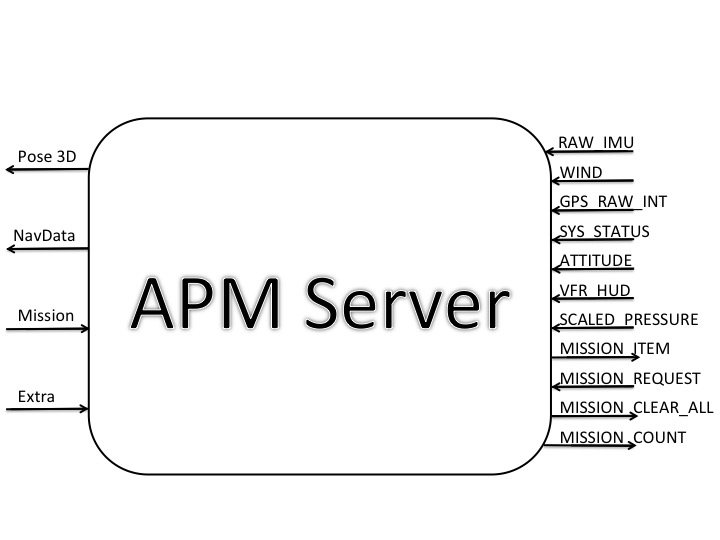
\includegraphics[scale=0.5]{img/diseno.jpg}
  \caption{Diseño de entradas y salidas de \texttt{APM Server}}
  \label{fig:diseno_apms_caja_negra}
\end{figure}

In order to adress it, a Python in \texttt{JdeRobot} component has been developed who implements all of above features called \texttt{APM Server}. 
\texttt{APM Server} is organized in three logical layers.
\begin{itemize}
\item Comunication's layer with APM's devices. ensures the establishment and maintenance the comunication with the APM device through \texttt{MAVLink's} commands.
\item Bussiness Layer. In this layer the driver convert form \texttt{MAVLink's} commands to ICE interfaces objects and viceversa.
\item \texttt{JdeRobot comunication's layer} This layer create all the ICE servers needed and handle incoming and outgoing ICE interfaces objects.
\end{itemize}
\begin{figure}[h]
\centering{
   \label{f:diseno_apms_caja_trans}
    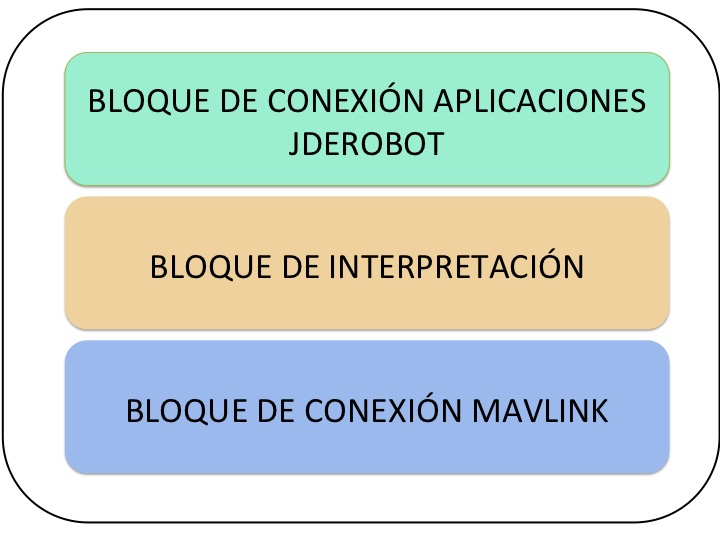
\includegraphics[width=0.7\textwidth]{img/diseno1.jpg}}
    \caption{Bloques del driver \texttt{APM Server}}
  
\end{figure}

\section{Comunication's layer with APM's devices}
\label{sec:apm_comunication}
% Always give a unique label
% and use \ref{<label>} for cross-references
% and \cite{<label>} for bibliographic references
% use \sectionmark{}
% to alter or adjust the section heading in the running head

In this layer the driver send the \texttt{MAVLink's} commands and recieve the \texttt{MAVLink's} messages which conform the comunication with the APM device.
The driver have to understand the APM device's messages received in \texttt{MAVLink} protocol as well as build this commands and send it to the APM.

\subsection{MAVLink's message}

The driver handle 11 commands of the full set of \texttt{MAVLink's} commands (see Figure 3.1) to allow the \texttt{JdeRobot} integration. Below it's described one of them in order to know this protocol.

\begin{verbatim}
<message id="33" name="GLOBAL_POSITION_INT">
	<description>The filtered global position 
	(e.g. fused GPS and accelerometers). The 
	position is in GPS-frame (right-handed, Z-up).
	It is designed as scaled integer message 
	since the resolution of float is not 
	sufficient.	</description>
<field type="uint32_t" name="time_boot_ms" units="ms">
	Timestamp (milliseconds since system boot)</field>
<field type="int32_t" name="lat" units="degE7">Latitude, 
	expressed as degrees * 1E7</field>
<field type="int32_t" name="lon" units="degE7">Longitude, 
	expressed as degrees * 1E7</field>
<field type="int32_t" name="alt" units="mm">Altitude in 
	meters, expressed as * 1000 (millimeters)</field>
<field type="int32_t" name="relative_alt" units="mm">
	Altitude above ground in meters, expressed as 
	* 1000 (millimeters)</field>
<field type="int16_t" name="vx" units="cm/s">Ground X 
	Speed (Latitude, positive north), expressed as 
	m/s * 100</field>
<field type="int16_t" name="vy" units="cm/s">Ground Y 
	Speed (Longitude, positive east), expressed as 
	m/s * 100</field>
<field type="int16_t" name="vz" units="cm/s">Ground Z 
	Speed (Altitude, positive down), expressed 
	as m/s * 100</field>
<field type="uint16_t" name="hdg" units="cdeg">Vehicle 
	heading (yaw angle) in degrees * 100, 0.0..359.99 
	degrees. If unknown, set to: UINT16_MAX</field>
</message>
\end{verbatim}

One example of this incoming message is:
\begin{verbatim}
GLOBAL_POSITION_INT {time_boot_ms : 480614, lat : -
353632612, lon : 1491652301, alt : 584110, 
relative_alt : -179, vx : 0, vy : 0, vz : 0, hdg : 
35608}
\end{verbatim}

\subsection{Setup and APM connection}

As has been showed the APM comunication is under \texttt{MAVLink} so the setup and conection have its own commands in this protocol.
To help us to build and understand these messages the driver uses \texttt{pymavlink}.

The connection is established in the server object creation, in the \_\_init\_\_() method of the class. The connection command needs two parameters: the device and the connection speed in bauds.
{\scriptsize
\begin{lstlisting}
classServer:
	def__init__(self,port,baudrate):
		self.master=mavutil.mavlink_connection(port,
					baudrate,autoreconnect=True)
		self.master.wait_heartbeat()
		...
__init__()
#test=Server("/dev/ttyUSB0",57600)#ConnectiontotherealAPMdevice
test=Server("udp:192.168.1.133:14558",57600)#ConnectiontoSITL
\end{lstlisting}}

The last two sentences shows an example of a real device connection and SITL's connection respectively.

Once the connection is made, the AMP \texttt{MAVLink's} messages start to be stored in a buffer, and we can setup it. The incoming messages rate and the set of these command we need are configurable parameters. Set up it is easy as is showed in the following lines.

{\scriptsize
\begin{lstlisting}
RATE=50
self.master.mav.request_data_stream_send(self.master.target_system,
						self.master.target_component,
						mavutil.mavlink.MAV_DATA_STREAM_ALL,
						RATE,1)
\end{lstlisting}}

The available set connections are:

\begin{verbatim}
MAV_DATA_STREAM_ALL	Enable all data streams
MAV_DATA_STREAM_RAW_SENSORS	Enable IMU_RAW, 
	        GPS_RAW, GPS_STATUS packets.
MAV_DATA_STREAM_EXTENDED_STATUS	Enable GPS_STATUS, 
	        CONTROL_STATUS, AUX_STATUS
MAV_DATA_STREAM_RC_CHANNELS	Enable RC_CHANNELS_SCALED,
	        RC_CHANNELS_RAW, SERVO_OUTPUT_RAW
MAV_DATA_STREAM_RAW_CONTROLLER	Enable 
	        ATTITUDE_CONTROLLER_OUTPUT, 
	        POSITION_CONTROLLER_OUTPUT, 
	        NAV_CONTROLLER_OUTPUT.
MAV_DATA_STREAM_POSITION	Enable LOCAL_POSITION, 
	        GLOBAL_POSITION/GLOBAL_POSITION_INT messages.
MAV_DATA_STREAM_EXTRA1	Dependent on the autopilot
MAV_DATA_STREAM_EXTRA2	Dependent on the autopilot
MAV_DATA_STREAM_EXTRA3	Dependent on the autopilot

\end{verbatim}

And the RATE value depends of the choosed device.


\subsection{APM data reading}
\label{subsec:apm_data_reading}

In order to retrieve the APM sensors measures, a thread is ejecuting a message handler all the time.
In this handler the method search for seven types of messages (like GLOBAL\_POSITION\_INT) which contains the needed data to fill the two ICE interfaces that the server serves: \texttt{Pose3D} y \texttt{NavData}.


\subsection{Sending missions to APM}
\label{sec:mission_apm}

This is the most important part of the driver. The driver recieve two ICE interfaces, one developed in this project called \texttt{mission} with the waypoints to follow and the \texttt{Extra} interface with the take off and land maneuvers.
Once a mission is received through these interfaces objects, \texttt{APM Server} build the \texttt{MAVLink's} commands needed to sent it to the APM. To perform it, a new thread with a listener was developed in order to know if there is a incominf mission.
Once this listener detects an incoming mission, call to \texttt{setMission(self, mission)} who build the \texttt{MAVLink's} commands and sent it as the Figure 3.3 diagram shows.
The \texttt{setMission(self, mission)} method read througth the list of waypoints and if \texttt{takeOffDecision} and \texttt{landDecision} of \texttt{Extra} object are seted to True add the \texttt{MAVLink's} commands of take off and land at first and last of the list of commans whitch is sended to the APM.
 

\begin{figure}[H]
  \centering
  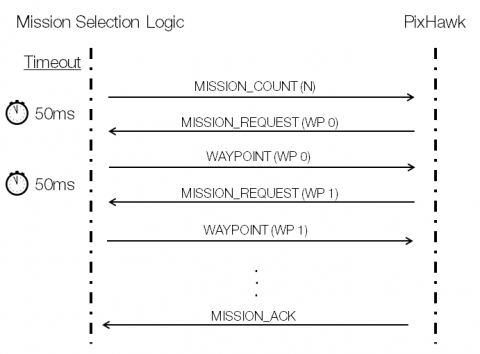
\includegraphics[scale=0.70]{img/waypoint-protocol-sendlist.png}
  \caption{\texttt{MAVLink's} missions sending protocol}
  \label{fig:misiones_mavlink}
\end{figure}

\section{JdeRobot's conection layer}
\label{sec:apm_jderobot_comunication}

In this layer all the ICE interfaces objects are handled. The driver uses four interfaces. Two of there are served (outgoing), \texttt{Pose3D} and \texttt{NavData} and the rest are received: \texttt{mission} and \texttt{extra}.
Each interfaces has its own thread with its own ICE server (note that ICE servers communication are bidirectional, so in this case ``server'' word don't refer to the side of the data).
In the following lines an ICE server implementation are showed.
{\scriptsize
\begin{lstlisting}

def openPose3DChannel(self, pose3D):
   status = 0
   ic = None
   Pose2Tx = pose3D
   try:
       ic = ICE.initialize(sys.argv)
       adapter = ic.createObjectAdapterWithEndpoints("Pose3DAdapter", 
       				"default -p 9998")
       object = Pose2Tx
       adapter.add(object, ic.stringToIdentity("ardrone_pose3d")) 
       adapter.activate()
       ic.waitForShutdown()
   except:
       traceback.print_exc()
       status = 1
   if ic:
       try:
           ic.destroy()
       except:
           traceback.print_exc()
           status = 1
   sys.exit(status)
\end{lstlisting}}

\section*{Interpretation layer}
\label{interpretation_layer}

This layer makes all the needed data's tranformation. So once the \texttt{MAVLink's} message is located, this layer makes it fit in the corresponding ICE interfaces and the same in opposite side communication. 
The \texttt{setMission(self, mission)} and the \texttt{refreshAPMPose3D()} and
\texttt{refreshAPMnavdata()} are the most important methods involved in this layer.

%%%%%%%%%%%%%%%%%%%%%%%% referenc.tex %%%%%%%%%%%%%%%%%%%%%%%%%%%%%%
% sample references
% %
% Use this file as a template for your own input.
%
%%%%%%%%%%%%%%%%%%%%%%%% Springer-Verlag %%%%%%%%%%%%%%%%%%%%%%%%%%
%
% BibTeX users please use
% \bibliographystyle{}
% \bibliography{}
%
\biblstarthook{In view of the parallel print and (chapter-wise) online publication of your book at \url{www.springerlink.com} it has been decided that -- as a genreral rule --  references should be sorted chapter-wise and placed at the end of the individual chapters. However, upon agreement with your contact at Springer you may list your references in a single seperate chapter at the end of your book. Deactivate the class option \texttt{sectrefs} and the \texttt{thebibliography} environment will be put out as a chapter of its own.\\\indent
References may be \textit{cited} in the text either by number (preferred) or by author/year.\footnote{Make sure that all references from the list are cited in the text. Those not cited should be moved to a separate \textit{Further Reading} section or chapter.} The reference list should ideally be \textit{sorted} in alphabetical order -- even if reference numbers are used for the their citation in the text. If there are several works by the same author, the following order should be used: 
\begin{enumerate}
\item all works by the author alone, ordered chronologically by year of publication
\item all works by the author with a coauthor, ordered alphabetically by coauthor
\item all works by the author with several coauthors, ordered chronologically by year of publication.
\end{enumerate}
The \textit{styling} of references\footnote{Always use the standard abbreviation of a journal's name according to the ISSN \textit{List of Title Word Abbreviations}, see \url{http://www.issn.org/en/node/344}} depends on the subject of your book:
\begin{itemize}
\item The \textit{two} recommended styles for references in books on \textit{mathematical, physical, statistical and computer sciences} are depicted in ~\cite{science-contrib, science-online, science-mono, science-journal, science-DOI} and ~\cite{phys-online, phys-mono, phys-journal, phys-DOI, phys-contrib}.
\item Examples of the most commonly used reference style in books on \textit{Psychology, Social Sciences} are~\cite{psysoc-mono, psysoc-online,psysoc-journal, psysoc-contrib, psysoc-DOI}.
\item Examples for references in books on \textit{Humanities, Linguistics, Philosophy} are~\cite{humlinphil-journal, humlinphil-contrib, humlinphil-mono, humlinphil-online, humlinphil-DOI}.
\item Examples of the basic Springer style used in publications on a wide range of subjects such as \textit{Computer Science, Economics, Engineering, Geosciences, Life Sciences, Medicine, Biomedicine} are ~\cite{basic-contrib, basic-online, basic-journal, basic-DOI, basic-mono}. 
\end{itemize}
}

\begin{thebibliography}{99.}%
% and use \bibitem to create references.
%
% Use the following syntax and markup for your references if 
% the subject of your book is from the field 
% "Mathematics, Physics, Statistics, Computer Science"
%
% Contribution 
\bibitem{science-contrib} Broy, M.: Software engineering --- from auxiliary to key technologies. In: Broy, M., Dener, E. (eds.) Software Pioneers, pp. 10-13. Springer, Heidelberg (2002)
%
% Online Document
\bibitem{science-online} Dod, J.: Effective substances. In: The Dictionary of Substances and Their Effects. Royal Society of Chemistry (1999) Available via DIALOG. \\
\url{http://www.rsc.org/dose/title of subordinate document. Cited 15 Jan 1999}
%
% Monograph
\bibitem{science-mono} Geddes, K.O., Czapor, S.R., Labahn, G.: Algorithms for Computer Algebra. Kluwer, Boston (1992) 
%
% Journal article
\bibitem{science-journal} Hamburger, C.: Quasimonotonicity, regularity and duality for nonlinear systems of partial differential equations. Ann. Mat. Pura. Appl. \textbf{169}, 321--354 (1995)
%
% Journal article by DOI
\bibitem{science-DOI} Slifka, M.K., Whitton, J.L.: Clinical implications of dysregulated cytokine production. J. Mol. Med. (2000) doi: 10.1007/s001090000086 
%
\bigskip

% Use the following (APS) syntax and markup for your references if 
% the subject of your book is from the field 
% "Mathematics, Physics, Statistics, Computer Science"
%
% Online Document
\bibitem{phys-online} J. Dod, in \textit{The Dictionary of Substances and Their Effects}, Royal Society of Chemistry. (Available via DIALOG, 1999), 
\url{http://www.rsc.org/dose/title of subordinate document. Cited 15 Jan 1999}
%
% Monograph
\bibitem{phys-mono} H. Ibach, H. L\"uth, \textit{Solid-State Physics}, 2nd edn. (Springer, New York, 1996), pp. 45-56 
%
% Journal article
\bibitem{phys-journal} S. Preuss, A. Demchuk Jr., M. Stuke, Appl. Phys. A \textbf{61}
%
% Journal article by DOI
\bibitem{phys-DOI} M.K. Slifka, J.L. Whitton, J. Mol. Med., doi: 10.1007/s001090000086
%
% Contribution 
\bibitem{phys-contrib} S.E. Smith, in \textit{Neuromuscular Junction}, ed. by E. Zaimis. Handbook of Experimental Pharmacology, vol 42 (Springer, Heidelberg, 1976), p. 593
%
\bigskip
%
% Use the following syntax and markup for your references if 
% the subject of your book is from the field 
% "Psychology, Social Sciences"
%
%
% Monograph
\bibitem{psysoc-mono} Calfee, R.~C., \& Valencia, R.~R. (1991). \textit{APA guide to preparing manuscripts for journal publication.} Washington, DC: American Psychological Association.
%
% Online Document
\bibitem{psysoc-online} Dod, J. (1999). Effective substances. In: The dictionary of substances and their effects. Royal Society of Chemistry. Available via DIALOG. \\
\url{http://www.rsc.org/dose/Effective substances.} Cited 15 Jan 1999.
%
% Journal article
\bibitem{psysoc-journal} Harris, M., Karper, E., Stacks, G., Hoffman, D., DeNiro, R., Cruz, P., et al. (2001). Writing labs and the Hollywood connection. \textit{J Film} Writing, 44(3), 213--245.
%
% Contribution 
\bibitem{psysoc-contrib} O'Neil, J.~M., \& Egan, J. (1992). Men's and women's gender role journeys: Metaphor for healing, transition, and transformation. In B.~R. Wainrig (Ed.), \textit{Gender issues across the life cycle} (pp. 107--123). New York: Springer.
%
% Journal article by DOI
\bibitem{psysoc-DOI}Kreger, M., Brindis, C.D., Manuel, D.M., Sassoubre, L. (2007). Lessons learned in systems change initiatives: benchmarks and indicators. \textit{American Journal of Community Psychology}, doi: 10.1007/s10464-007-9108-14.
%
%
% Use the following syntax and markup for your references if 
% the subject of your book is from the field 
% "Humanities, Linguistics, Philosophy"
%
\bigskip
%
% Journal article
\bibitem{humlinphil-journal} Alber John, Daniel C. O'Connell, and Sabine Kowal. 2002. Personal perspective in TV interviews. \textit{Pragmatics} 12:257--271
%
% Contribution 
\bibitem{humlinphil-contrib} Cameron, Deborah. 1997. Theoretical debates in feminist linguistics: Questions of sex and gender. In \textit{Gender and discourse}, ed. Ruth Wodak, 99--119. London: Sage Publications.
%
% Monograph
\bibitem{humlinphil-mono} Cameron, Deborah. 1985. \textit{Feminism and linguistic theory.} New York: St. Martin's Press.
%
% Online Document
\bibitem{humlinphil-online} Dod, Jake. 1999. Effective substances. In: The dictionary of substances and their effects. Royal Society of Chemistry. Available via DIALOG. \\
http://www.rsc.org/dose/title of subordinate document. Cited 15 Jan 1999
%
% Journal article by DOI
\bibitem{humlinphil-DOI} Suleiman, Camelia, Daniel C. O�Connell, and Sabine Kowal. 2002. `If you and I, if we, in this later day, lose that sacred fire...�': Perspective in political interviews. \textit{Journal of Psycholinguistic Research}. doi: 10.1023/A:1015592129296.
%
%
%
\bigskip
%
%
% Use the following syntax and markup for your references if 
% the subject of your book is from the field 
% "Computer Science, Economics, Engineering, Geosciences, Life Sciences"
%
%
% Contribution 
\bibitem{basic-contrib} Brown B, Aaron M (2001) The politics of nature. In: Smith J (ed) The rise of modern genomics, 3rd edn. Wiley, New York 
%
% Online Document
\bibitem{basic-online} Dod J (1999) Effective Substances. In: The dictionary of substances and their effects. Royal Society of Chemistry. Available via DIALOG. \\
\url{http://www.rsc.org/dose/title of subordinate document. Cited 15 Jan 1999}
%
% Journal article by DOI
\bibitem{basic-DOI} Slifka MK, Whitton JL (2000) Clinical implications of dysregulated cytokine production. J Mol Med, doi: 10.1007/s001090000086
%
% Journal article
\bibitem{basic-journal} Smith J, Jones M Jr, Houghton L et al (1999) Future of health insurance. N Engl J Med 965:325--329
%
% Monograph
\bibitem{basic-mono} South J, Blass B (2001) The future of modern genomics. Blackwell, London 
%
\end{thebibliography}

